\documentclass[margin=1mm]{standalone}

\usepackage{tikz}
\usepackage{fontspec}
\setmainfont{QTHeidelbergType}

\begin{document}
	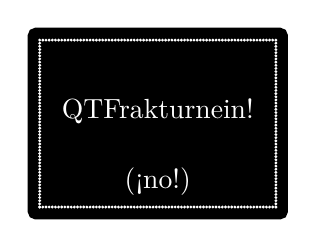
\begin{tikzpicture}		
		\fill (-1.55,-1.28) rectangle (1.55, 0.96);
		
		\node at (0,0) [white] {\fontsize{40}{40}\setmainfont{QTFraktur}nein!};
		\node at (0,-0.9) [white] {(¡no!)};
		
		\foreach \y in {-1.22, -1.18, ..., 0.9}
		{
			\fill [white] (-1.5,\y) circle (0.2mm);
			\fill [white] (1.5,\y) circle (0.2mm);
		}
		
		\foreach \x in {-1.5, -1.46, ..., 1.5}
		{
			\fill [white] (\x,-1.22) circle (0.2mm);
			\fill [white] (\x,0.9) circle (0.2mm);
		}
	
		\draw [line width=3, rounded corners = 1.5] (-1.6,-1.325) rectangle (1.6,1.005);
		
	\end{tikzpicture}
\end{document}